\begin{center}
    \section*{BAB 3 METODOLOGI}
\end{center}

\setcounter{section}{3}
\setcounter{subsection}{0}

\subsection{Alur Kerja Proyek}
    \begin{figure}[htp]
         \centering
         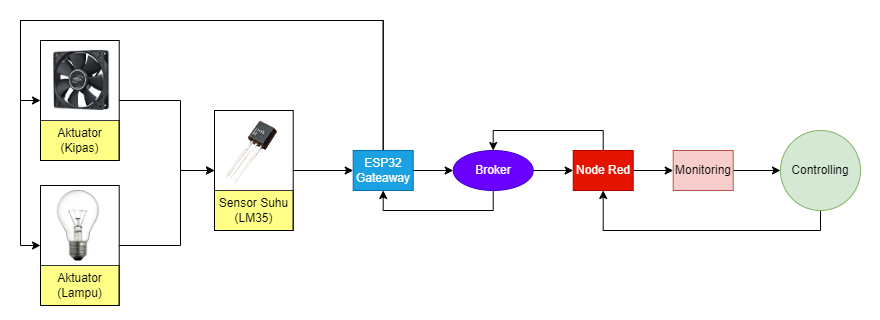
\includegraphics[width=15cm]{image/Diagram Cara Kerja.png}
         \label{fig:alur kerja}
         \caption{Alur Kerja Proyek}
    \end{figure}

\subsection{Penjelasan Alur Kerja}
    \begin{itemize}
        \item Sensor LM35 membaca suhu dalam kotak dengan tegangan yang dia dapatkan berdasarkan suhu. Semakin panas suhu dalam kotak, maka voltasenya makin tinggi. Sebaliknya, semakin dingin suhu dalam kotak, maka voltasenya makin rendah.
        \item ESP32 menerima data suhu dari sensor LM35 dengan cara membaca sinyal analog yang diberikan oleh sensor suhu LM35. Sinyal analog tersebut kemudian diubah menjadi sinyal digital
        \item Broker (Raspberry Pi) menerima sinyal digital yang diberikan oleh ESP32
        \item Subscriber (Node Red) meminta data sinyal digital dari broker untuk memonitoring data suhu tersebut. 
        \item Setelah meminta data suhu dari broker, akan dilihat apakah suhu dalam kotak terlalu dingin atau terlalu panas. Jika terlalu dingin, maka kita akan atur agar lampu menyala. Sebaliknya, jika terlalu panas, maka kita akan atur agar kipas yang menyala.
        \item Setelah controlling tersebut, Node Red yang sebelumnya menjadi subscriber, sekarang menjadi broker untuk mengirim salah satu perintah tadi ke Raspberry Pi, yang mana sekarang menjadi subscriber.
        \item Raspberry Pi tadi menerima perintah, dan menerjemahkan perintah tersebut agar dapat dibaca oleh ESP32 sebagai perintah kepada aktuator, antara lampu yang menyala atau kipas yang menyala.
        \item Salah satu aktuator akan menyala untuk menyesuaikan suhu dalam kotak tersebut agar tetap stabil.
    \end{itemize} 
    